\chapter{Introduction}

The Zero-Hunger Goal, one of 17 Sustainable Development Goals, seeks to "end hunger, achieve food security and improved nutrition, and promote sustainable agriculture" by 2030 (\cite{united_nations_transforming_2015}). In reality, however, hunger and food insecurity have increased. By 2030, 512 million people could be chronically undernourished according to the projections of the Food and Agriculture Organization of the United Nations (\cite{noauthor_state_2026}). There are many causes of this crisis, all of which will be exacerbated by climate change. The link between climate change and food security is clear. Loss of biodiversity, soil degradation, and water pollution hinder the development of efficient, resilient food production systems by reducing agricultural productivity and crop yields, impacting food availability and prices while reducing accessibility for vulnerable populations. Current food systems are not prepared for these challenges, yet they must meet rising food demand: to meet projected needs, by 2050, agricultural production will need to increase by 60\%, and by nearly 100\% in developing countries (\cite{leal_filho_sustainable_2022}).
\\


Barley (\textit{Hordeum vulgare}) is a major cereal crop, making up 19\% of the EU’s harvested cereal production (\cite{european_commission_agricultural_2025}). It is mainly used as feed for livestock and in malt production, but holds great potential for further nutritional applications. Compared to other crops, barley tolerates relatively high heat, which makes it a promising candidate crop for climate resilience efforts (\cite{soare_survey_2023}). However, heat tolerance alone does not address the full range of pressures outlined above: yield stability, nutrient-use efficiency, and disease resistance remain limiting factors even in climate-adapted crops. Realising barley's potential therefore requires complementary strategies that enhance resilience and promote productivity.
\\


Beyond plant genetic engineering, another innovative approach to improving productivity while stabilising agricultural systems against climate change is the manipulation of a crop's rhizosphere microbiota (\cite{wang_narrow-spectrum_2025}). Unlike breeding or genetic modification, microbiome-based interventions can be applied to existing cultivars without altering the plant genome itself. By harnessing beneficial soil microbes’ functions such as carbon sequestration, improved water retention, protection against (a-)biotic stressors and promoted plant growth, they help to mitigate the effects of climate change (Compant et al., 2025; \cite{jansson_soil_2020}). Plant-growth promoting microbes specifically support their host, for example by enhancing plant metabolism via the production and secretion of phytohormones, fixing N\textsubscript{2}, increasing nitrogen and phosphorus uptake, and competing with/suppressing pathogenic microbes (\cite{ansabayeva_plant_2025}). 
\\


Studying the properties of microbiomes can be difficult \textit{in planta}, mainly due to the constantly changing environment and unknown culture conditions. Synthetic Communities (SynComs) offer a reliable, reductionist approach. These communities are composed of selected bacterial strains that together represent a simplified version of the microbiome while retaining functional traits. When analysed via genome-scale modelling, SynComs reduce biological complexity on one hand, while on the other allow the investigation of larger and more complex communities than what would be tractable \textit{in vitro}. SynComs are a promising system for the analysis of underlying mechanisms of microbial interaction, prediction of metabolic fluxes, interspecies exchanges as well as the identification of keystone strains. The data obtained through such analyses is a valuable basis for further model validation and hypothesis testing (\cite{feierabend_silico_2025}). 
\\


The stable composition of microbial communities is especially important given their roles in biofertilisation and stress tolerance (\cite{chem_towards_2025, qi_higher_2026}), yet the multifaceted drivers of community stability are subject of ongoing research and debate. A stable community does not imply a constant composition between species at every time point. Rather, it represents the community's average state over time. This means that no organism consistently outperforms all others and dominates the entire community, additionally stability does not necessarily require the persistence of every member: if a strain’s function is redundant with remaining members, such that overall community function remains unchanged, this strain may not be essentially required for long-term stability (\cite{allison_resistance_2008}). Stability indicators are the occurrence of reciprocal dependencies, the response to additions/removals of community members and the presence keystone species (\cite{butler_stability_2018, liu_keystone_2025, wang_narrow-spectrum_2025, zelezniak_metabolic_2015}). 
\\


\cite{mahdi_low_2026}, established two SynComs in the barley (\textit{Hordeum vulgare L.}) rhizosphere. These communities differ in their assembly approach: the core community is assembled based on co-occurrence, whereas the trait-optimised community is constructed from strains previously shown to promote plant growth and pathogen protection. They show that the trait-optimised community reduces plant root growth and is generally less stable and balanced. The core community however exhibits stable and balanced interactions, without reducing plant growth. While \cite{mahdi_low_2026} established these phenotypic differences, the underlying metabolic principles driving them remain unresolved. This thesis addresses this gap using computational approaches to model the metabolism of these two barley rhizosphere SynComs, core and trait (plant-growth) optimised, collected from the barley rhizosphere. I investigate these systems to understand the impact of different assembly strategies on community behaviour. The goal is to improve the design of SynComs and tap their full potential in maximising barley productivity and protection. 

Specifically, I aim to answer the following questions: 
\begin{enumerate}
    \item Do the reconstructed and curated genome-scale metabolic models meet current community quality standards? 
    \item How do individual strains and communities differ in metabolic principles governing interactions such as substrate utilisation, metabolite exchange (cross-feeding), and metabolic niche occupation?
    \item Can keystone species be identified within each community?
    \item Which stability indicators can be found within the communities?
    \item How is community behaviour impacted by the SynCom assembly strategy?
\end{enumerate}

\begin{figure}[htbp]
  \centering
  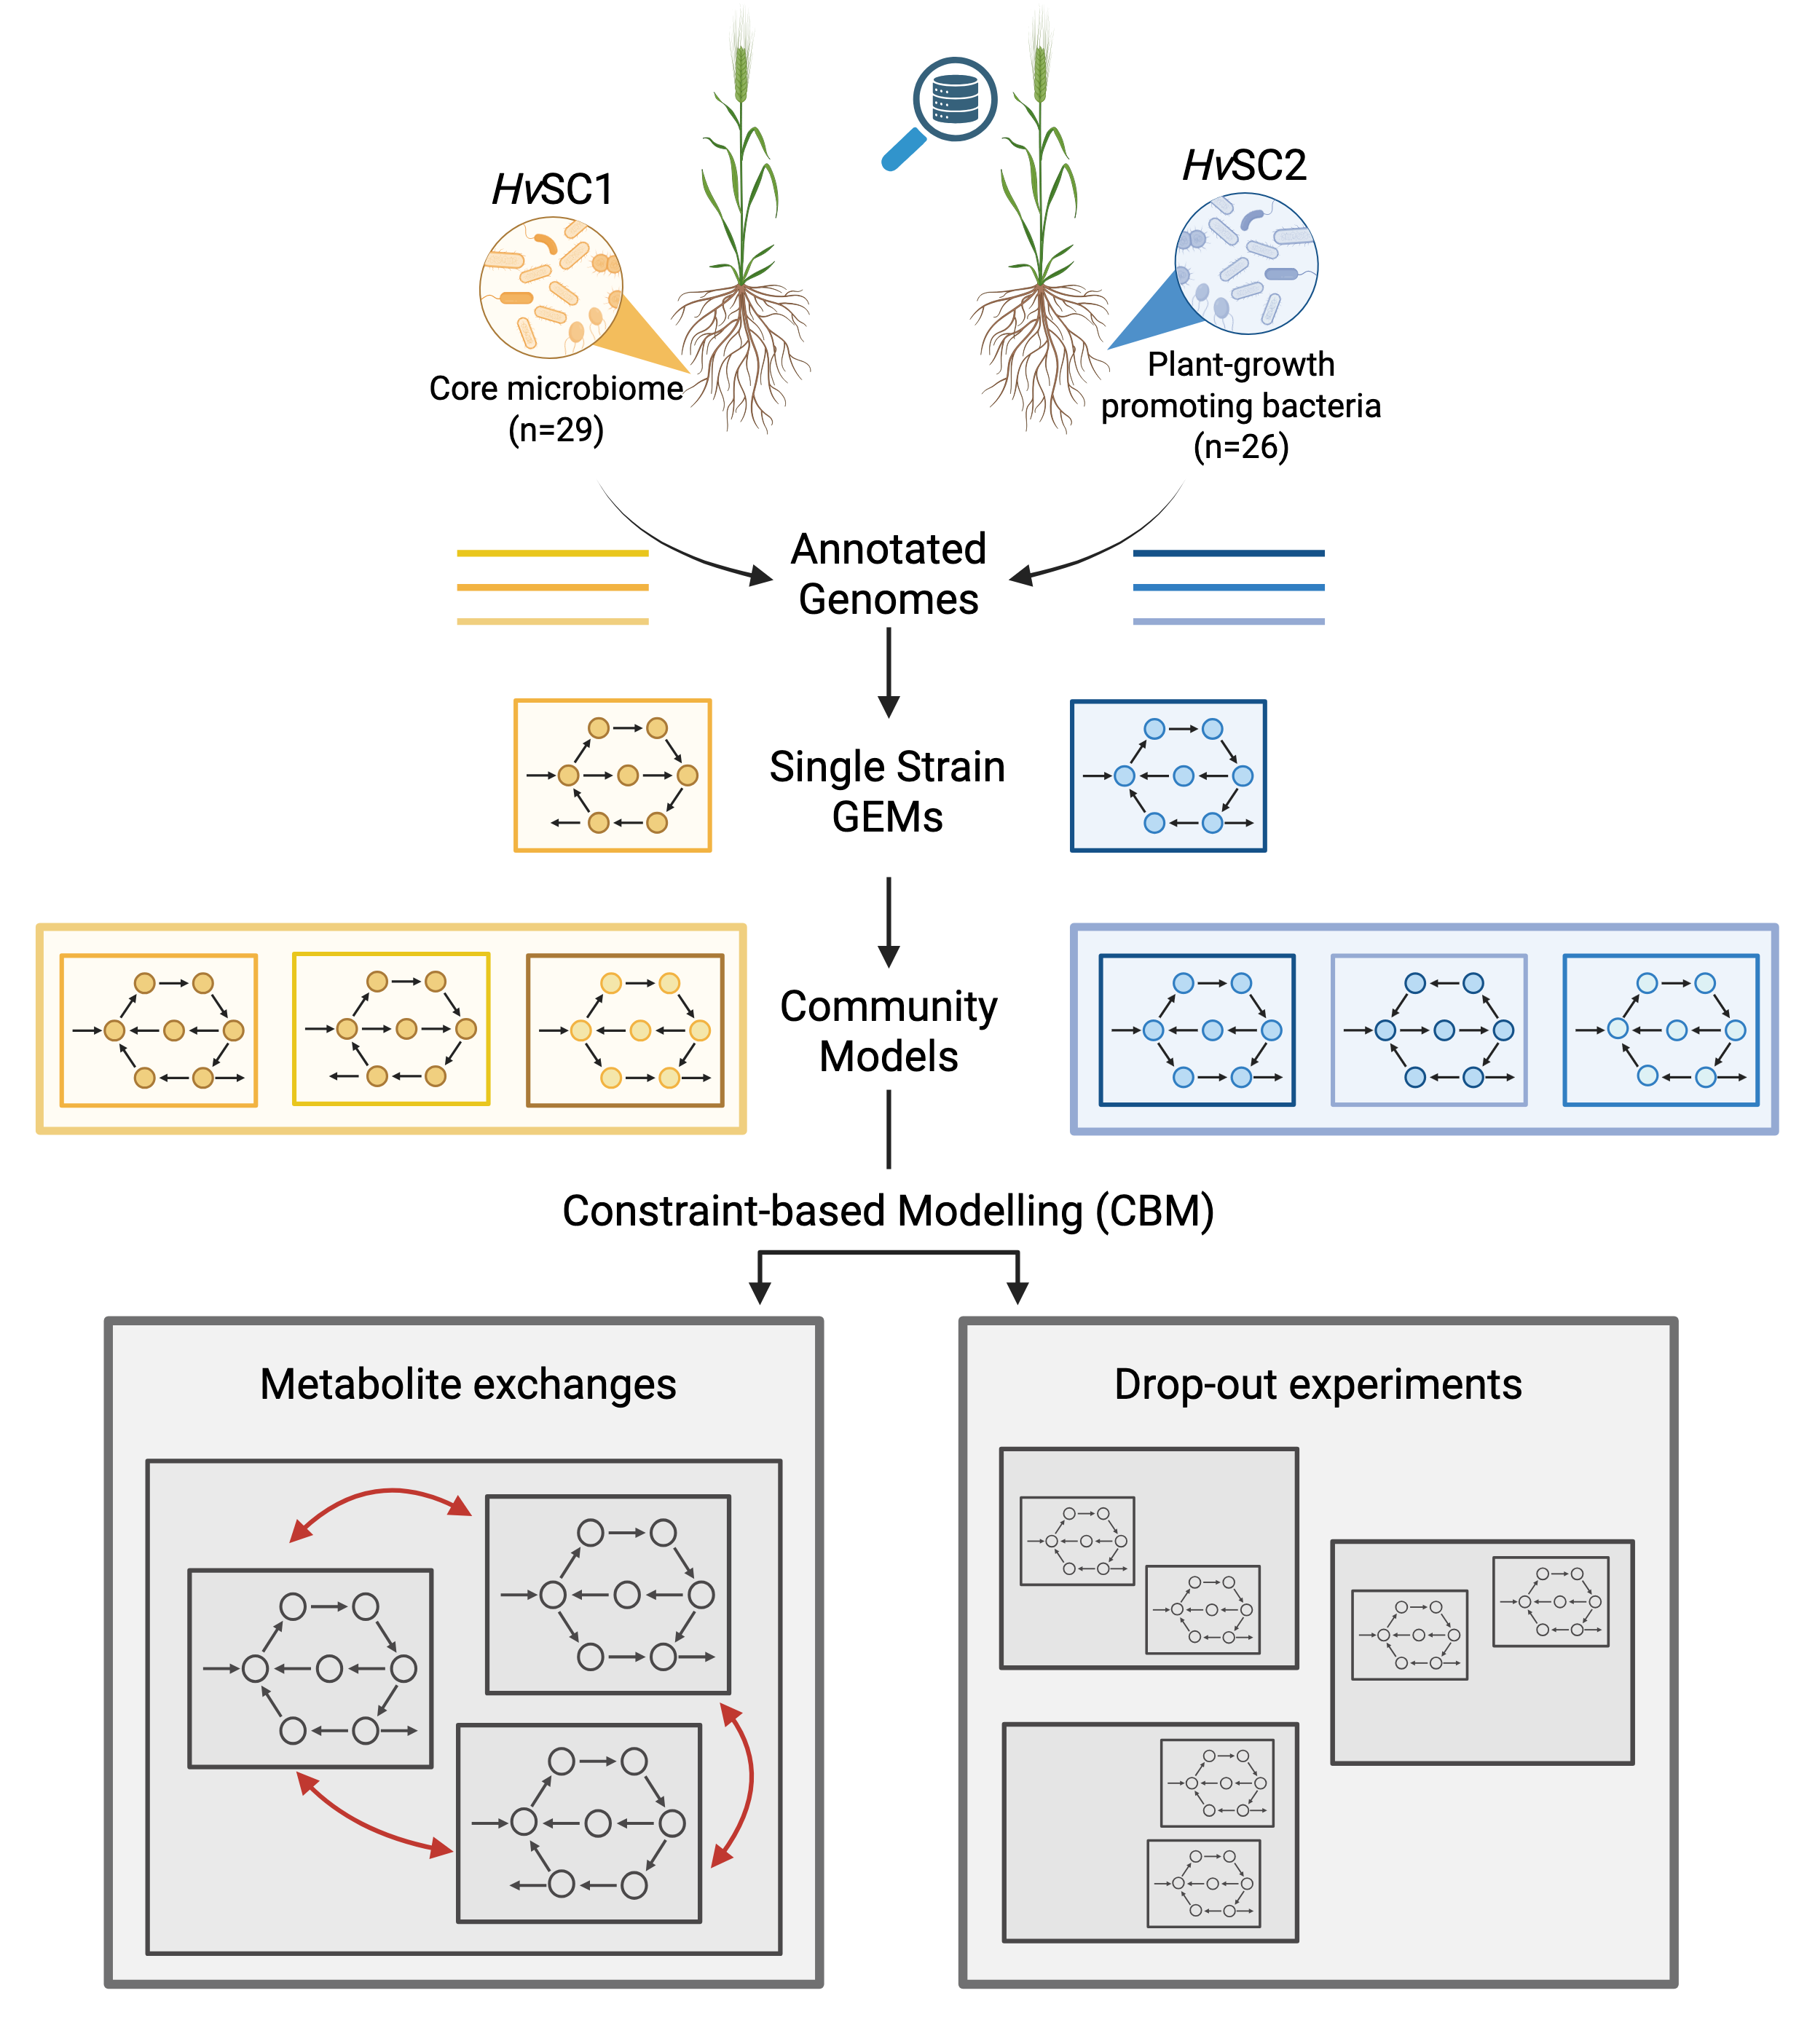
\includegraphics[width=1\textwidth]{fig/Graphical_abstract.png}
  \caption[Graphical abstract of the reconstruction and analysis workflow]{Graphical abstract of the reconstruction and analysis workflow. First, single strain genome-scale metabolic models (GEMs) were reconstructed from annotated genomes and assembled into community models. Using constraint-based modelling (CBM), metabolic behaviour, metabolite exchanges and drop-out experiments were evaluated. Created with BioRender.}
  \label{fig:graphical_abstract}
\end{figure}

The structure of this thesis follows the graphical abstract, as depicted in Figure \ref{fig:graphical_abstract}. 
